\chapter{Getting started}

\section{An Introduction}
This template was created by Junjie Li, the primary contributor, and Manuel Liu Wang, the secondary contributor, both UB students majoring in computer science. It is not an official template from UB.

It can be an essay, thesis, report, or article. The template is for broad usage. Mathematical notation, matrix application, pictures, formulas, a range of word styles, and page size are all included.


\section{Tutorial}
Options \underline{[Option1, Option2, Option3, Option4, Option5, and Option6]} are listed in the first line. , those options regulate the template's fundamental layout: Option 1 modifies the page mode; Option 2 sets the font size; Option 3 establishes the page side; Option 4 applies the desired font style; Option 5 toggles the print/online version; and Option 6 activates the draft option.

On the other side, there is the optional zone, which you can omit if you choose. For instance, the first optional zone has the cover and the footer.


\section{Usage}

You can look at the chapter sections, beginning with section 2, to get a quick overview of how to use this template. All the chapters have usage examples.    




\chapter{My second Chapter}


\section{Images exemple}


\begin{figure}[H]
    \centering
    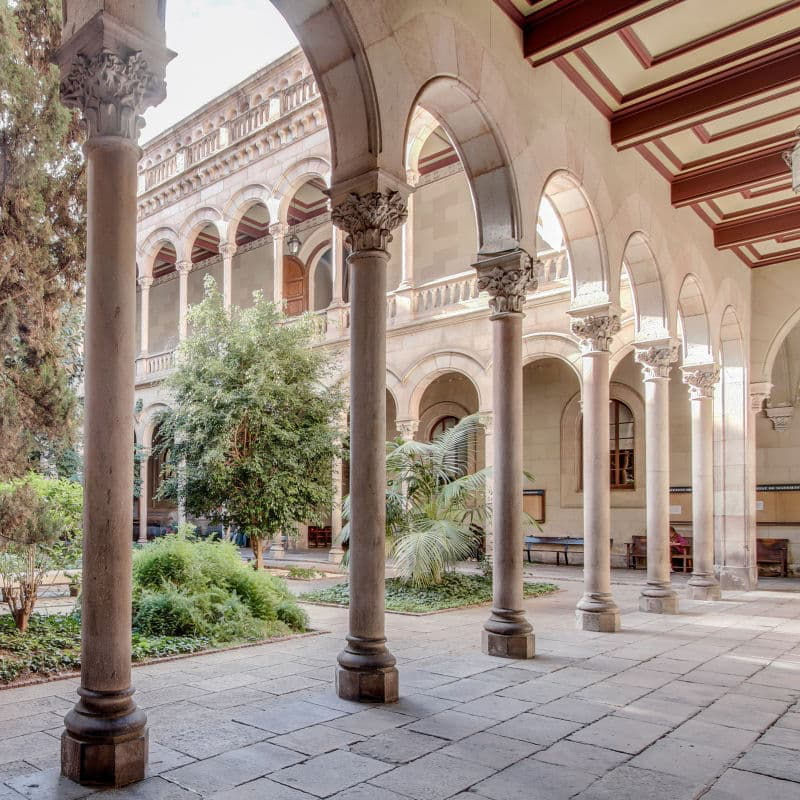
\includegraphics[width=6cm, height=4cm]{images/edifici-historic-universitat-de-barcelona.jpg}
    \caption{Images example}
    \label{taula}
\end{figure}%



\begin{figure}[H]
    \centering
    \begin{minipage}[t]{0.48\textwidth}
        \centering
        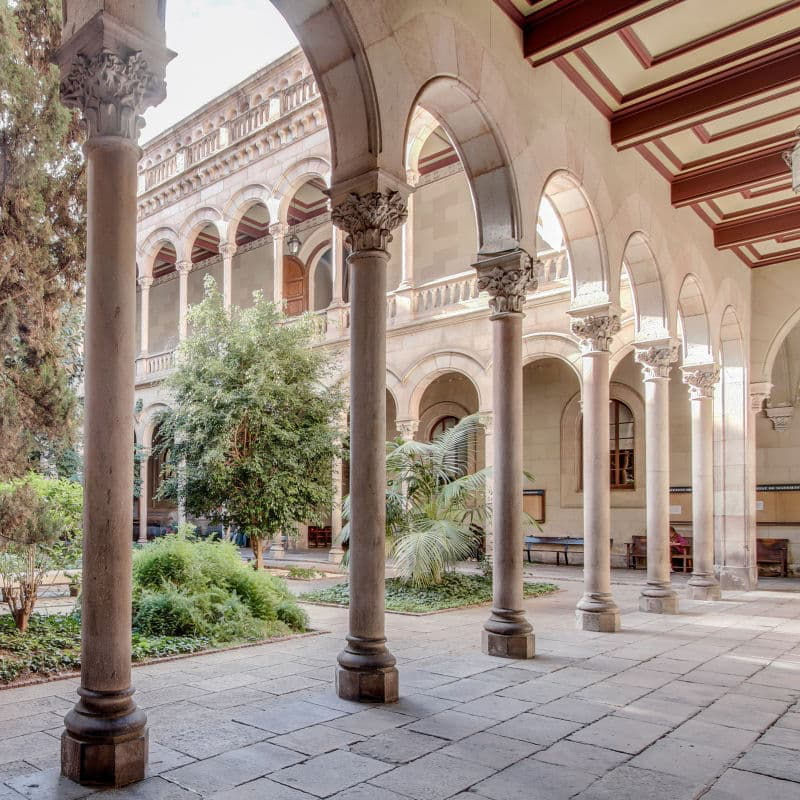
\includegraphics[width=6cm, height=4cm]{images/edifici-historic-universitat-de-barcelona.jpg}
        \caption{Images example2}
    \end{minipage}
    \begin{minipage}[t]{0.48\textwidth}
        \centering
        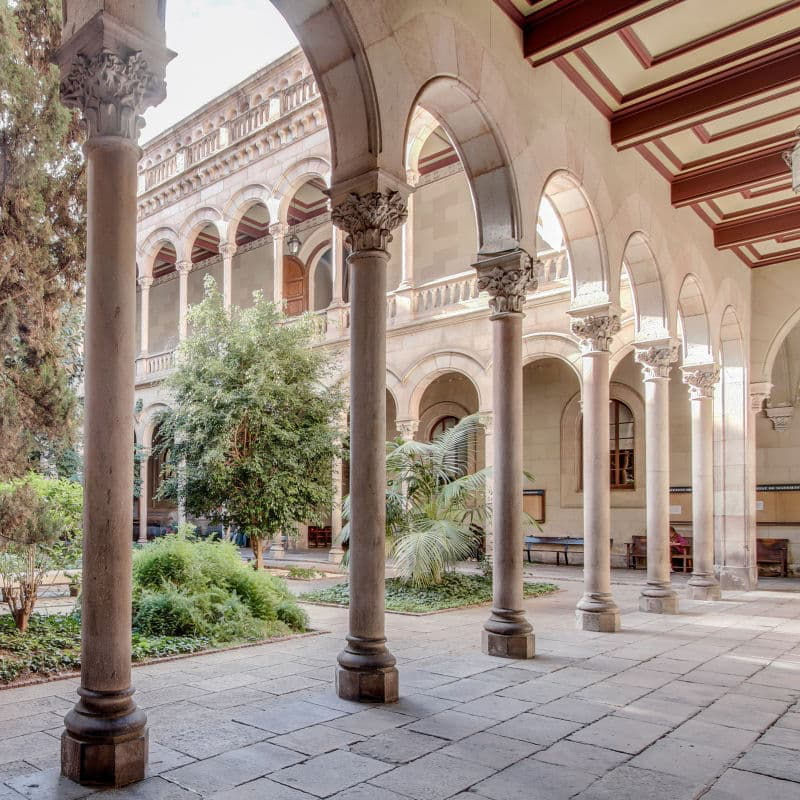
\includegraphics[width=6cm, height=4cm]{images/edifici-historic-universitat-de-barcelona.jpg}
        \caption{Images example3}
    \end{minipage}
\end{figure}


\section{Math example}

Example math equation on the sentence:

The most famous equation in the world: $E^2 = (m_0c^2)^2 + (pc)^2$, which is 
known as the \textbf{energy-mass-momentum} relation as an in-line equation.


Example math equation on the squart:

\begin{equation}
P_{R_X} = P_{T_X} \cdot G_{T_X}  \cdot G_{R_X} \cdot \left( \frac{\lambda}{4\pi d} \right)^2  \cdot \eta
\end{equation}

\section{Table example}

\begin{table}[H]
\caption{A badly formatted table}
\centering
\label{table:bad_table}
\begin{tabular}{|l|c|c|c|c|}
\hline 
& \multicolumn{2}{c}{Species I} & \multicolumn{2}{c|}{Species II} \\ 
\hline
Dental measurement  & mean & SD  & mean & SD  \\ \hline 
\hline
I1MD & 6.23 & 0.91 & 5.2  & 0.7  \\
\hline 
I1LL & 7.48 & 0.56 & 8.7  & 0.71 \\
\hline 
I2MD & 3.99 & 0.63 & 4.22 & 0.54 \\
\hline 
I2LL & 6.81 & 0.02 & 6.66 & 0.01 \\
\hline 
CMD & 13.47 & 0.09 & 10.55 & 0.05 \\
\hline 
CBL & 11.88 & 0.05 & 13.11 & 0.04\\ 
\hline 
\end{tabular}
\end{table}



\begin{table}[H]
\caption{A nice looking table}
\centering
\label{table:nice_table}
\begin{tabular}{l c c c c}
\hline 
\multirow{2}{*}{Dental measurement} & \multicolumn{2}{c}{Species I} & \multicolumn{2}{c}{Species II} \\ 
\cline{2-5}
  & mean & SD  & mean & SD  \\ 
\hline
I1MD & 6.23 & 0.91 & 5.2  & 0.7  \\

I1LL & 7.48 & 0.56 & 8.7  & 0.71 \\

I2MD & 3.99 & 0.63 & 4.22 & 0.54 \\

I2LL & 6.81 & 0.02 & 6.66 & 0.01 \\

CMD & 13.47 & 0.09 & 10.55 & 0.05 \\

CBL & 11.88 & 0.05 & 13.11 & 0.04\\ 
\hline 
\end{tabular}
\end{table}


It high recommended to use {\url{https://www.tablesgenerator.com/#}} to generate easy table.




\chapter{My third chapter}

Write your conclusion here.






\chapter{Glossary tutorial}

 The \Gls{latex} typesetting markup language is specially suitable 
for documents that include \gls{maths}. Give



\chapter{bibliograp Tutorial}

Using you can display a bibliography divided into sections, depending on citation type. 
Let's cite! Einstein's journal paper \cite{einstein} and Dirac's book \cite{dirac} are physics-related items. 
Next, \textit{The \LaTeX\ Companion} book \cite{latexcompanion}, Donald Knuth's website \cite{knuthwebsite}, \textit{The Comprehensive Tex Archive Network} (CTAN) \cite{ctan} are \LaTeX-related items; but the others, Donald Knuth's items, \cite{knuth-fa,knuth-acp} are dedicated to programming.



\chapter{Exanple of Indices of terms}

In this example, several keywords\index{keywords} will be 
used which are important and deserve to appear in the 
Index\index{Index}.

Terms like generate\index{generate} and some\index{others} 
will also show up. Terms in the index can also be 
nested \index{Index!nested}